\chapter{Circuit Layout}
\label{sec:CircuitLayout}

\section{Dimensionierung der Widerst�nde}
\label{sec:Dimensionierung}

\section{Erstellen der Schaltung in PSpice (Viviane Bremer)}
\label{sec:PSpice}

Zur weiteren Dimensionierung der Auswerteelektronik ist die Schaltung in PSpice erstellt worden. Diese ist in Abbildung \ref{fig:PSpice1} dargestellt. Der linke Teil bis vor die zwei rechten Operationsverst�rker ist zur Offsetkompensation des Sensors gedacht. Der restliche Teil dient zur Signalverst�rkung. F�r die Widerst�nde werden als erste N�herung die in Kapitel \ref{sec:Dimensionierung} bestimmten Werte genutzt. In Kapitel \ref{sec:SimReal} werden die gleichen Schritte mit zur Verf�gung stehenden Bauteilen durchgef�hrt.


\begin{figure}[hb]
	
	\rotatebox{90}{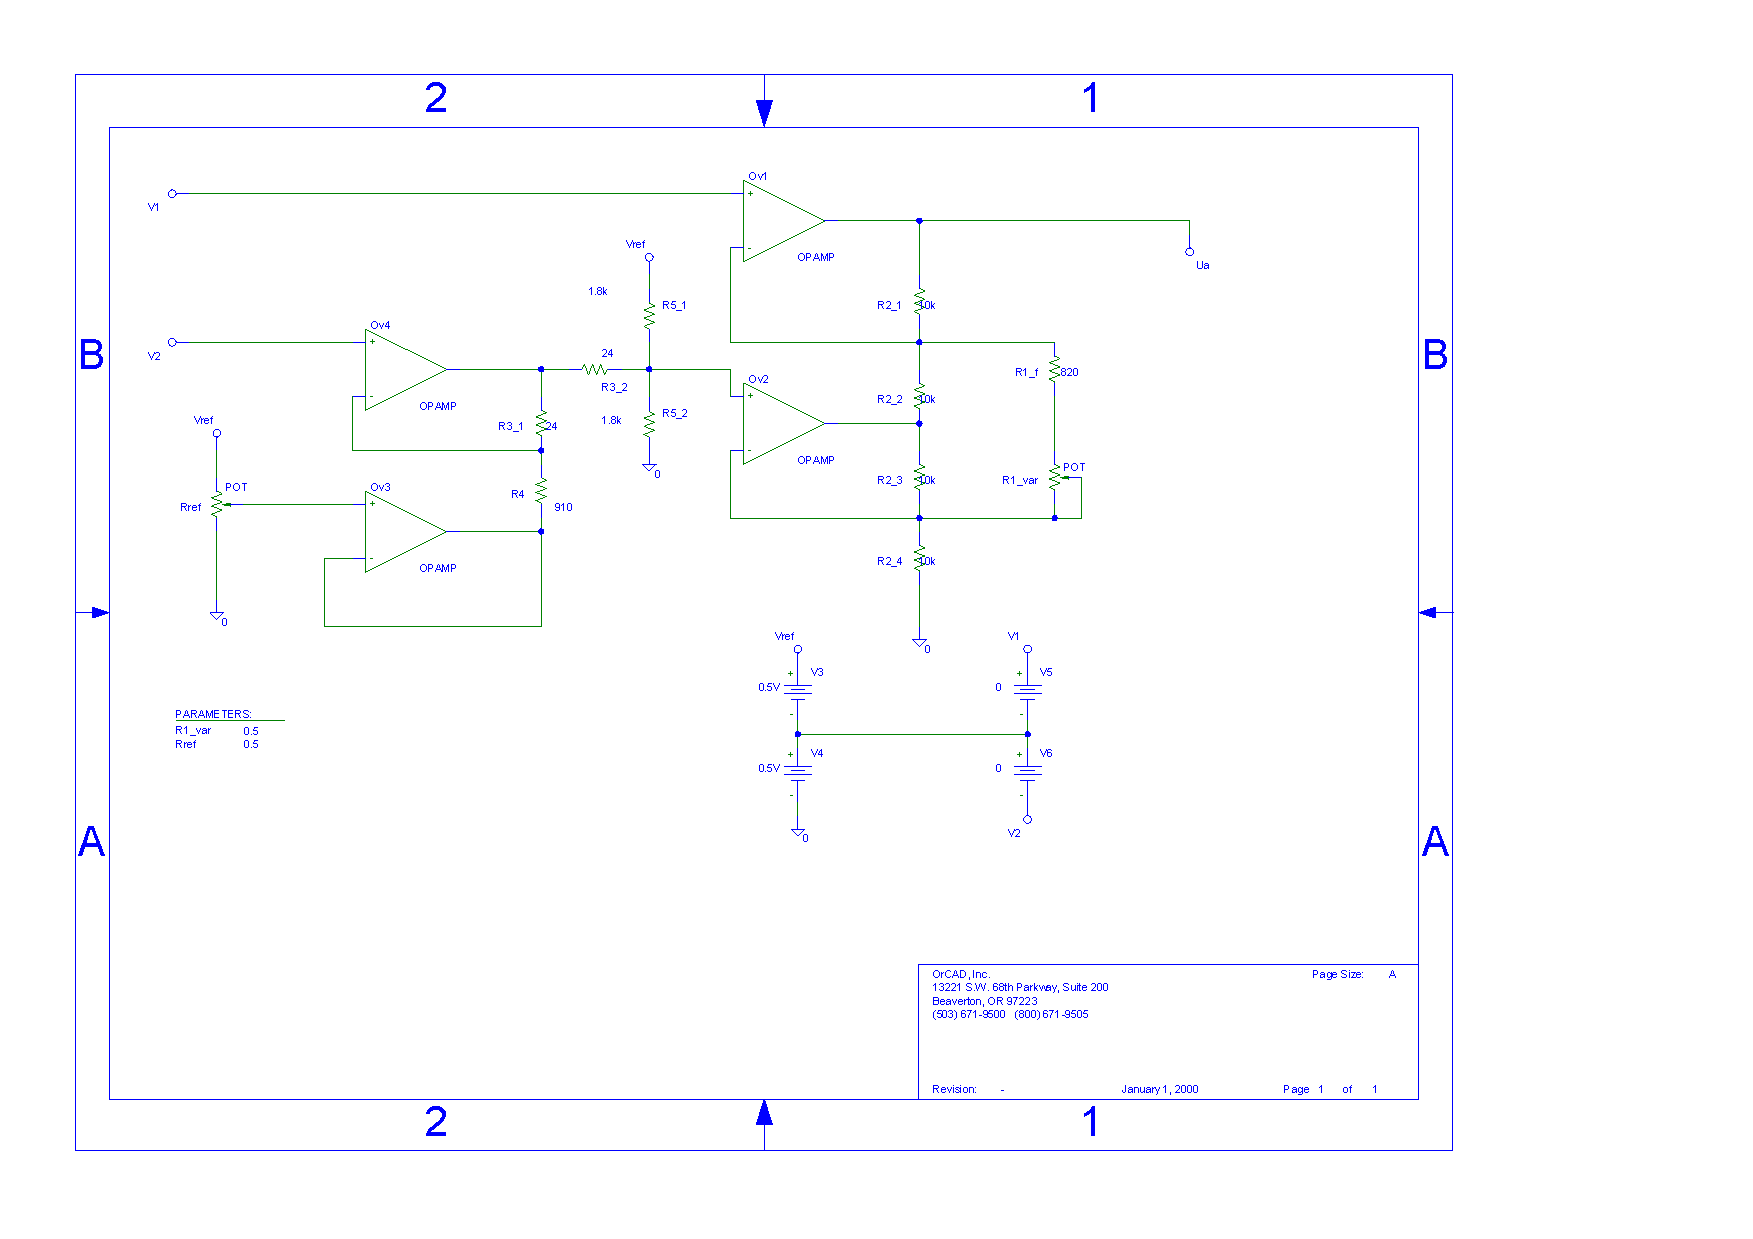
\includegraphics[trim = 10mm 10mm 50mm 12mm, clip,width=0.9\textheight]{figures/Schaltplan1.pdf}}
	\caption{Schaltplan der Auswerteelektronik in PSpice}\label{fig:PSpice1}
\end{figure}


\section{Simulation der Auswerteelektronik mit theoretisch berechneten Werten}
\label{sec:SimTheor}
\subsection{Einfluss des Offset-Potentiometers (Viviane Bremer)}
\label{sec:Offset-Poti}

Zun�chst wird nur das Offset-Potentiometer betrachtet. Daf�r wird der Wert des Potentiometers Rref von Null auf seinen Endwert erh�ht und die Potentialdifferenz von Eingangsspannung am Operationsverst�rker Ov\,2 und Eingangsspannung am Operationsverst�rker Ov\,4 �ber den Widerstand geplottet. Wie aus der Abbildung \ref{fig:Offset-Poti1} abzulesen ist, hat die Offsetkompensation einen Stellbereich von \unit[$\pm$12]{mV}.

\begin{figure}[hb]
	\centering
	\includegraphics[trim = 10mm 10mm 10mm 5mm, clip,width=0.9\textwidth]{figures/Simulation1_1.pdf}
	\caption{Verlauf der Spannungsdifferenz zwischen Operationsverst�rker Ov\,2 und Ov\,4 �ber dem Widerstand Rref}\label{fig:Offset-Poti1}
\end{figure}

\subsection{Einfluss des Verst�rkungs-Potentiometers (Viviane Bremer)}
\label{sec:gain-Poti}

Als n�chstes wird der Einfluss des Verst�rkungs-Potentiometers  $R1_{var}$ untersucht. Hierbei wird �hnlich vorgegangen, wie beim Offset-Potentiometer. Diesmal wird jedoch der Quotient aus Ausgangsspannung und Eingangsspannungsdifferenz genutzt. Das Ergebnis ist in Abbildung \ref{fig:gain-Poti1} zu sehen. Der Wertebereich der Verst�rkung liegt zwischen 21.8 und 25.6.

\begin{figure}[hb]
	\centering
	\includegraphics[trim = 10mm 10mm 10mm 5mm, clip,width=0.9\textwidth]{figures/Simulation1_2.pdf}
	\caption{Verlauf der Spannungsdifferenz zwischen Eingangs- und Ausgangsspannung �ber dem Widerstand $R1_{var}$}\label{fig:gain-Poti1}
\end{figure}

\subsection{Abgleichung der Schaltung (Viviane Bremer)}
\label{sec:Abgleich1}
Zum Schluss werden Rref und $R1_{var}$ zusammen variiert und die Eingangsspannung auf \unit[0]{V} gesetzt. Bei \unit[0]{V} sollte die Verst�rkung das Signal nicht beeinflussen, wenn der Offset ausgeglichen wurde.  In Abbildung \ref{fig:Abgleich1} ist zur Visualisierung die Ausgangsspannung �ber dem Widerstand aufgetragen.

\begin{figure}[hb]
	\centering
	\includegraphics[trim = 10mm 10mm 10mm 5mm, clip,width=0.9\textwidth]{figures/Simulation1_3.pdf}
	\caption{Verlauf der Ausgangsspannung �ber dem Widerstand}\label{fig:Abgleich1}
\end{figure}

\section{Simulation der Auswerteelektronik mit Bauteilwerten/Simulation with real values}
\label{sec:SimReal}

\section{Filter}